Let 
\begin{align}
\begin{split}
\vec{A} = \myvec{1 \\ 1}, 
\vec{B} = \myvec{3 \\ 5}, 
\vec{C} = \myvec{-2 \\ 4}, 
\vec{D} = \myvec{-1 \\ -5}. 
\end{split}
\end{align}
Then, 
\begin{align}
\brak{\vec{B} - \vec{A}}
    &= \myvec{3\\5} - \myvec{1\\1}
    = \myvec{2\\4}
\\
    \brak{\vec{D} - \vec{B}}
    &= \myvec{-1\\-5} - \myvec{3\\5}
    = \myvec{-4\\-10}
\\
     \brak{\vec{A} - \vec{D}}
    &= \myvec{1\\1} - \myvec{-1\\-5}
    = \myvec{2\\6}
\end{align}
%
Row reducing the matrix formed by the  vectors, 
\begin{equation}
\begin{math}
\myvec{2 & 4 & 1\\-4 & -10 & 1\\2 & 6 & 1\\}
\\
\implies 
\myvec{2 & 4 & 1\\-4 & -10 & 1\\2 & 6 & 1\\}
\xleftrightarrow[]{R_2\leftrightarrow R_3}
\myvec{2 & 4 & 1\\2 & 6 & 1\\-4 & -10 & 1\\}
\xleftrightarrow[]{R_3\leftrightarrow R_1+R_2+R_3}
\myvec{2 & 4 & 1\\2 & 6 & 1\\0 & 0 & 3\\}
\xleftrightarrow[]{R_2\leftrightarrow R_2-R_1}
\myvec{2 & 4 & 1\\0 & 2 & 0\\0 & 0 & 3\\}
\end{math}
\end{equation}
The number of non-zero rows in the matrix = 3. Hence the matrix
is full rank and  AB, BD, DA are not collinear.
See Fig. \ref{hem/2/9/1/fig:Quad ABCD}, which shows that the points given form a quadrilateral.
\begin{figure}[!ht]
    \centering
    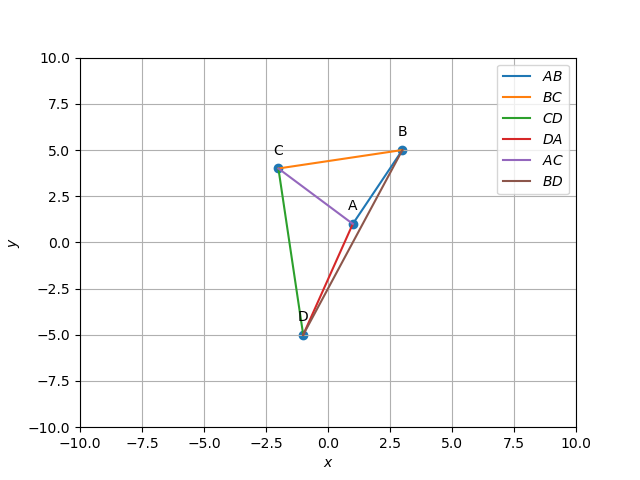
\includegraphics[width=\columnwidth]{2/solution/9/1/QUAD.png}
    \caption{Quadrilateral ABCD}
    \label{hem/2/9/1/fig:Quad ABCD}
\end{figure}
%
Area of a $\triangle ABC$ is given by
%
\begin{align}
\triangle ABC = 
\frac{1}{2}\mydet{
1 & 1 & 1\\1 & 3 & -2\\1 & 5 & 4\\}
= 9
\end{align}
%
Area of $\triangle ACD$  is given by
\begin{align}
\triangle ACD = 
\frac{1}{2}\mydet{
1 & 1 & 1\\1 & -2 & -1\\1 & 4 & -5\\}
= 11.5
\end{align}
Thus, the area of quadrilateral ABCD = 9+11.5 = 20.5.
